\chapter{State of art}\label{ch:stateofArt}
\noindent
Cooperative and non cooperative Sense and Avoid (SAA) systems are key enablers for Unmanned Aircraft (UAV) to routinely access non-segregated airspace \cite{spriesterbach2013unmanned}. Both cooperative and non-cooperative SAA systems are being developed to address this integration requirement.
\noindent
The SAA capability is defined as the automatic detection of possible conflicts by the UAV platform under consideration and performing avoidance maneuver tasks to prevent the identified collisions. An analysis of the available SAA candidate technologies and the associated sensors for both cooperative and non-cooperative SAA systems is presented in \cite{muraru2011critical}. Non-cooperative Collision Detection and Resolution (CD\&R) for UAV is considered as one of the major challenges that needs to be addressed \cite{lai2012see} for the insertion of UAVs in non-segregated air space. As a result, a number of non-cooperative sensors for the SAA system have been adopted. Light Detection and Ranging (LIDAR)is used for detecting, warning and avoiding obstacles for low-level flying \cite{sabatini2014lidar}.
\noindent
An approach to the definition of encounter models and their applications to SAA strategies is presented in \cite{kochenderfer2008encounter} for both cooperative and non-cooperative scenarios.
\noindent
Since 2014, there is a visible strong political support for developing rules on drones but regulations are not harmonized yet. The European Aviation Safety Agency (EASA) has been tasked to develop a regulatory framework for drone operations and proposals for the regulation of "low-risk" UAV operations. In achieving this, EASA is working closely with the Joint Authorities for Regulation of Unmanned Systes (JARUS) \cite{jarus2016regulations}.
\newpage
\section{UAV motion model}
\noindent
This section strongly follows \cite{lee2011structure}.

\subsection{Continuous-time systems}
%This is very imprecise. A good notation is:
%1. u is the control function. It is a map from a time interval to \R^p, i.e., u:[0,T] \to %\R^p. Thus you could write u\in \C^p
%2. u(t) is the value (in \R^p) of the control function u. It is correct to write u(t)\in %\R^p

%You have to say what \C^p is. I guess that you mean the space of continuous functions. If this is the case, this specification is very unnatural since this space is too restrictive. Controls of interest usually have discontinuities.  More common is L^1 (space of integrable functions).

\noindent Consider a class of systems given by functions:
\begin{equation}
    \begin{split}
    S&: \vec{u}(t)  \to \vec{x}(\vec{x}_0,t) \\
    \vec{u}&(t): [0,T] \to \R^p \\
    \vec{u}&(t)\in \mathbb{R}^p , \vec{x}(t) \in \mathbb{R}^n \\
    \end{split}
\end{equation}
where $\vec{u}(t)$ and  $\vec{x}(\vec{x}_0,t)$ are a sets of continuous-time signals.
These are often called continuous-time systems because they operate on
continuous-time signals. Frequently, such systems can be defined by differential
equations that relate the input signal to the output signal.
A prototypical description of a controlled (there is a control input signal)
continuous-time system is:
\begin{equation}\label{eq:nonlinearsystem}
    \dot{x}(t) = f(t,x(t),u(t)), u(t) \in U(t)
\end{equation}
where $f:\mathbb{R}\times\mathbb{R}^n\times\mathbb{R}^p\to\mathbb{R}^n$
satisfies the conditions for existence
and uniqueness of the ordinary differential equation and $u$ is our control\cite{butcher1987numerical}.

\subsection{Discrete-time systems}
\noindent
\noindent Consider another class of systems given by functions
\begin{equation}
    \begin{split}
    S&: \vec{u}(k)  \to \vec{x}(k), \\
    k& \in \{0, t_s, 2.t_s, 3.t_s, \dots i.t_s\}, i \in \N^+\\
    \vec{u}&(k)\in \mathbb{R}^p , \vec{x}(k) \in \mathbb{R}^n\\
    \end{split}
\end{equation}
where $\vec{u}(k), \vec{x}(k)$ is a set of discrete-time signals. They can be represented by a function $f$ like $f:\{0, t_s, 2.t_s, 3.t_s, \dots i.t_s\} \to \R^n,  i \in \N^+$ where $t_s$ is sampling time and $i$ is discrete step \cite{shampine1997matlab}.

%Optimal control
\section{Optimal control}
\noindent These section show how to arrive at an optimal decision assuming that complete information is given. The phrase complete information is given means that the following requirements are met:
\begin{enumerate}
    \item The \textit{set of all permissible decisions} is known.
    \item The \textit{cost of each decision} is known.
\end{enumerate}
\noindent When these conditions are satisfied, the decisions can be ranked according to whether they incur greater or lesser cost. An optimal decision is then any decision which incurs the least cost among the set of permissible decisions. \newpage\noindent In order to model a \textit{decision-making situation} in mathematical terms, certain further requirements must be satisfied:
\begin{enumerate}
    \item The \textit{set of all decisions} can be adequately represented as a subset of a vector space with each vector representing a decision.
    \item The \textit{cost corresponding to these decisions} is given by a real-valued function.
\end{enumerate}
\noindent Distinction between the function which is to be optimized and the functions which describe the constraints, although convenient for presenting the mathematical theory, may be quite artificial in practice. For instance, suppose chosen durations of various traffic lights in a section of a city so as to achieve optimum traffic flow. One can suppose that we know the transportation needs of all the people in this section. Before one can begin to suggest a design, one will need a \textit{criterion} to determine what is meant by \textit{optimum traffic flow}. More abstractly, one need a \textit{criterion} by which one can compare different decisions, which in this case are different patterns of traffic-light durations. One way of doing this is to assign as \textit{cost to each decision} the total amount of time taken to make all the trips within this section. An alternative and equally plausible goal may be to minimize the maximum waiting time (that is the total time spent at stop lights) in each trip. Now it may happen that these two objective functions may be inconsistent in the sense that they may give rise to different orderings of the permissible decisions. Indeed, it may be the case that the optimum decision according to the first criterion may be lead to very long waiting times for a few trips, so that this decision is far from optimum according to the second criterion. We can then redefine the problem as minimizing the first cost function (total time for trips) subject to the constraint that the waiting time for any trip is less than some reasonable bound (say one minute). In this way, the second goal (minimum waiting time) has been modified and reintroduced as a constraint. This interchangeability of goal and constraints also appears at a deeper level in much of the mathematical theory. One will see that in most of the results the objective function and the functions describing the constraints are treated in the same manner.

Given model of a single decision-maker with complete information can be generalized along other important direction. The hypothesis of complete information can be relaxed by allowing that decision-making occurs in an \textit{uncertain environment}.

Let say a person wants to invest 1,000 EUR in the stock market. One wants to maximize his capital gains, and at the same time minimize the risk of losing his money. The two objectives are incompatible, since the stock which is likely to have higher gains is also likely to involve greater risk. The situation is different,the outcome (future stock prices) is uncertain. It is customary to model this uncertainty stochastically. Thus, the investor may assign probability 0.5 to the event that the price of shares in Glamor company increases by 100 EUR, probability 0.25 that the price is unchanged, and probability 0.25 that it drops by 100 EUR. A similar model is made for all the other stocks that the investor is willing to consider, and a decision problem can be formulated as follows. How should 1,000 EUR be invested so as to maximize the expected value of the capital gains subject to the constraint that the probability of losing more than 100 EUR is less than 0.1 ? Same problem can be encountered with trajectory formulation model.

If the uncertainties are modelled stochastically as in the example above, then in many cases the techniques presented in this work can be usefully applied to the resulting optimal decision  problem. To do justice to these decision-making situations, however, it is necessary to give great attention to the various ways in which the uncertainties can be modelled mathematically. It is necessary to finding equivalent but simpler formulations. For instance, it is of great significance to know that, given appropriate conditions, an optimal decision problem under uncertainty is equivalent to another optimal decision problem under complete information. (This result, known as the \textit{Certainty-Equivalence principle} in economics has been extended the \textit{Separation Theorem} in the control literature. \cite{wonham1968matrix}) Unfortunately, to be able to deal with these models, one will need a good background in Statistics and Probability Theory besides the material presented in this work. We can only refer the reader to the extensive literature on \textit{Statistical Decision Theory} \cite{savage1954problem,blackwell19541954} and on \textit{Stochastic Optimal Control}
\cite{meditch1969stochastic,kushner1971introduction}

\subsection{Problem formulation}\label{s:problemOptT}
\noindent The general problem is considered in the form (\ref{eq:p65}), for simplicity purpose sample time $t_i$ will be considered in this chapter as $i$, system state $\vec{x}(t_i)$ will be denoted as $x(i)$ and system input $\vec{u}(t_i)$ will be denoted as $u(i)$.
\begin{equation}\label{eq:p65}
    \begin{aligned}
    &\text{Maximize } \sum_{i=0}^{N-1}f_0(i,x(i),u(i))\\
    &\text{subject to:}\\
    &\textit{Dynamics: } x(i+1) - x(i) = f(i,x(i),u(i)),i=0,\dots, N-1\\
    &\textit{Initial condition: } q_0(x(0) \le 0, g_0(x(0)) = 0\\
    &\textit{Final condition: } q_N(x(N)\le 0, g_N(x(N))) = 0\\
    &\textit{State-space constraint: } q_i(x(i))\le 0,\quad i = 1,\dots,N-1\\
    &\textit{Control constraint: } h_i(u_i)\le 0,\quad i = 1,\dots,N-1\\
    \end{aligned}
\end{equation}

\noindent Here $x(i)\in\R^n$, $u(i) \in \R^p$, $f_0(i,\cdot,\cdot): \R^{n+p}\to \R$, $f(i,\cdot,\cdot):\R^{n+p}\to\R^n$, $q_i: \R^n\to\R^{m_i}$, $g_i:\R^n\to\R^{l_i}$, $h_i: \R^p\to\R^{s_i}$ are given differentiable functions. This notation follows control terminology, $x(i)$ is \textit{system state} at time $i$ and $u(i)$ is the \textit{control input} at time $i$.
Using theorem from \cite{wonham1968matrix}, one can construct Lagrangian function $L$ as follows:
\begin{equation}
    \begin{split}
    L&\left( x(0),\dots,x(N);u(0),\dots,u(N-1);p(0),\dots,p(N); \right. \\
    &\left. \lambda^0,\dots,\lambda^N;\alpha^0,\dots,\alpha^N;\gamma^0,\dots,\gamma^{N-1} \right) =\\
    &\sum_{i=0}^{N-1} f_0(i,x(i),u_i) - \left\{ \sum_{i=0}^{N-1} (p(i+1)^T (x(i+1)-x(i) - f(i,x(i),u(i))) \right. \\
    &\left. \sum_{i=0}^N (\lambda^i)^T q_i(x(i)) + (\lambda^0)^T g_n(x(N)) + \sum_{i=0}^{N-1} (\gamma^i)^T h_i(u(i)) \right\}
    \end{split}
\end{equation}
\noindent Suppose that \textit{Constraint qualification} is satisfied for (\ref{eq:p65}) and $x^*(0),\dots,x^*(N)$; $u^*(0),\dots,u(N-1)$ is an optimal solution. Then by using Kuhn-Tucker Theorem \cite{kampas2005tricks}, there exist $p^*(i)\in\R^N$ for $1\le i \le N$, $\lambda^{i_*} \ge 0 \in \R^,$ for $0\le i \le N$, $\alpha^{i_*}\in \R^{l_i}$ for $0\le i \le N$, and $\gamma^{i_*} \ge 0 \in \R^{s_i}$ such that:
\begin{enumerate}
\item The derivative of $L$ evaluated at these points vanishes.
\item $\lambda^{i_*}q_i(x^*(i))=0$ for $0\le i \le N$, $\gamma^{i_*}h_i(u^*(i))=0$ for $0 \ le i \le N-1$
\end{enumerate}
\newpage\noindent Differentiating $L$ with respect to $x(0)$ gives:
\begin{equation}\label{eq:p66a}
    \begin{split}
    f_{0x}&(0,x^*(0),u^*(0)) - \{-(p^*(1))^T-(p^*(1))^T f(0,x^*(0),u*(0))\\
    & + (\lambda^{0_*})^T q_{0x}(x^*(0)) + (\lambda^{0_*})^T g_{0x}(x^*(0))\} = 0
    \end{split}
\end{equation}
\begin{equation}\label{eq:p66b}
    \begin{split}
    p^*(0) - p^*(1) &= f_x(0,x^*(0),u^*(0))^T p^*(1)\\
    &+ f_{0x}(0,x^*(0),u^*(0))^T - q_{0x}(x^*(0))^T \lambda^{0_*}
    \end{split}
\end{equation}
\noindent where $p*(0)$ is defined as:
\begin{equation}\label{eq:p67}
    p^*(0) = g_{0x}(x^*(0))^T \lambda^{0_*}
\end{equation}
\noindent Differentiating $L$ with respect to $x(i)$, $1\le i \le N-1$ and rearranging terms gives:
\begin{equation}
    \begin{split}\label{eq:p68}
    p^*(i) - p^*(i+1) &= f_x(i,x^*(i),u^*(i))^T p^*(i+1)\\
    & + f_{0x}(i,x^*(i),u^*(i))^T - q_{ix}(x^*(i))^T \lambda^{N_*}
    \end{split}
\end{equation}
\noindent Differentiating $L$ with respect to $x(N)$ gives:
\begin{equation}\label{eq:p69}
    p^*(N) = -g_N(x^*(N))^T \alpha^{N_*} - q_{N_x}(x^*(N))^T \lambda^{N_*}
\end{equation}
\noindent For convenience $\alpha^{N_*}$ can be replaced by $-\alpha^{N_*}$, therefore differentiating $L$ with respect to $x(N)$ gives:
\begin{equation}
    p^*(N) = g_N(x^*(N))^T \alpha^{N_*} - q_{N_x}(x^*(N))^T \lambda^{N_*}
\end{equation}
\noindent Differentiating $L$ with respect to $u(i)$, $0\le i \le N-1$ gives:
\begin{equation}\label{eq:p610}
    f_{0u}(i,x^*(i),u^*(i))^T + f_u(i,x^*(i),u^*(i))^T p^*(i+l)- h_{iu}(u^*(i))^T \gamma^{i_*} = 0
\end{equation}
\noindent Hamiltonian function $H$ is given by:
\begin{equation}
    H(i,x,u,p) = f_0(i,x,u) + p^T f(i,x,u)
\end{equation}
\noindent The dynamic equations for $0 \le i \le N-1$ then become:
\begin{equation}
    x^*(i+1) - x^*(i) = H_p(i,x^*(i),u^*(i),p^*(i+1))^T
\end{equation}
\noindent The adjoint equations (\ref{eq:p66a}, \ref{eq:p66b}, \ref{eq:p68}) for $0 \le i \le N-1$ then become:
\begin{equation}
    p^*(i) - p^*(i+1) = H_x(i,x^*(i),u^*(i),p^*(i+1))^T - q_{ix}(x^*(i))^T \lambda^{i_*}
\end{equation}
\noindent Then (\ref{eq:p610}) becomes for $0 \le i \le N-1$ as follow:
\begin{equation}
    h_{iu}(u^*(i))^T \gamma^{i_*} = H_{u}(i,x^*(i),u^*(i),p^*(i+1))^T
\end{equation}
\noindent If dynamic equations of original solution are linearized for $0 \le i \le N-1$  following linear model is obtained:
\begin{equation}
    \delta x(i+1) - \delta x(i) = f_x(i,x^*(i),u^*(i))\delta x(i) + f_u (i,x^*(i),u^*(i))\delta u(i)
\end{equation}
\noindent Homogeneous part is given as:
\begin{equation}
    z(i+1)- z(i) = f_x(i, x^*(i),u^*(i)) z(i)
\end{equation}
\noindent Which has for it an adjoint system:
\begin{equation}\label{eq:p613}
    r(i) - r(i+1) = f_x(i, x^*(i),u^*(i))^T r(i+1)
\end{equation}
\noindent Since the homogeneous part of the linear difference equations (\ref{eq:p66a}, \ref{eq:p66b}, \ref{eq:p68}) is (\ref{eq:p613}), we call (\ref{eq:p66a}, \ref{eq:p66b}, \ref{eq:p68}), the adjoint equations, and the $p^*(i)$ are called \textit{adjoint variables}.

If the $f_0(i,\cdot,\cdot)$ for time $0 \le i \le N-1$ are concave and the remaining functions in (\ref{eq:p65}) are linear then \textit{Constraint Qualification} is satisfied and the necessary conditions are also sufficient. Furthermore in this case one can see from (\ref{eq:p613}) that $u^*(i)$ is an optimal solution of:
\begin{equation}
    \begin{split}
        &\text{Maximize } H(i,x^*(i),u,p^*(i+1)).\\
        &\text{Subject to } h_i(u)\le 0.
    \end{split}
\end{equation}
\noindent For this reason the result is sometimes called the \textit{maximum principle}.

The conditions (\ref{eq:p67}, \ref{eq:p69}) are called \textit{transversality conditions} for the following reason. Suppose $q_0 \equiv 0$, $q_N \equiv 0$ so that initial and final conditions read $g_0(x(0))=0$, $g_N(x(N))=0$ which describes surfaces of state space $\R^n$. Conditions (\ref{eq:p67},\ref{eq:p69}) become respectively $p*(0) = g_{0x}(x^*(0))^T \alpha^{0_*}$, $p^*(N)= g_{Nx}(x^*(N))^T \alpha^{N_*}$, which means that $p^*(0)$ and $p^*(N)$ are respectively orthogonal or transversal to the initial and final surfaces.

\subsection{Minimum Principle} 
\noindent Main reason of this section is to show some classical minimum principle which gives reader overview of minimum principle mechanics and its relations to discrete time mechanisms discussed in sections \ref{s:problemOptT} and \ref{s:dynap}.
The principle was first known as Pontryagin's minimum principle and its proof is historically based on minimizing the \textit{Pontryagin function} $H$. The initial application of this principle was to the maximization of the terminal speed of a rocket. However, as it was subsequently mostly used for minimization of a performance index it has here been referred to as the minimum principle. Pontryagin's book solved the problem of minimizing a performance index \cite{pontryagin1962matematicheskaya}.
\noindent
Here the necessary conditions are shown for minimization of a functional. Take x to be the state of the dynamical system with input u, such that:
\begin{equation}
    \dot {x}=f(x,u),\quad x(0)=x_{0},\quad u(t)\in U,\quad t\in [t_0,T]
\end{equation}
Where $U$ is the set of admissible controls and $T$ is the terminal  time of the system. The control $u\in U$ must be chosen for all $t\in [t_0,T]$ to minimize the objective functional $J$ which is defined by the application and can be abstracted as following equation:
\begin{equation}
    J=\Psi (x(T))+\int _{0}^{T}L(x(t),u(t))\,dt
\end{equation}
The constraints on the system dynamics can be adjoined to the \textit{integrand of cost function} $L$ by introducing time-varying Lagrange multiplier vector $\lambda$ , whose elements are called the costates of the system. This motivates the construction of the Pontryagin function $H$ defined for all $t\in [t_0,T]$ by equation:
\begin{equation}
    {\displaystyle H(x(t),u(t),\lambda (t))=\lambda ^{\rm {T}}(t)f(x(t),u(t))-L(x(t),u(t))\,}
\end{equation}
\newpage\noindent \textit{Pontryagin's minimum principle} states that the optimal state trajectory $x^{*}$, optimal control $u^{*}$, and corresponding Lagrange multiplier vector $\lambda^*$ must minimize the \textit{Pontryagin function} $H$ so that following condition holds:
\begin{enumerate}
    \item $H(x^{*}(t),u^{*}(t),\lambda ^{*}(t),t)\leq H(x^{*}(t),u,\lambda ^{*}(t),t)$ for all time $t\in [0,T]$ and for all permissible control inputs $u \in U$.
    \item $\Psi _{T}(x(T))+H(T)=0$ in addition to previous condition.
    \item ${-{\dot {\lambda }}^{\rm {T}}(t)=H_{x}(x^{*}(t),u^{*}(t),\lambda (t),t)=\lambda ^{\rm {T}}(t)f_{x}(x^{*}(t),u^{*}(t))+L_{x}(x^{*}(t),u^{*}(t))}$ must be\\ satisfied. If the final state $x(T)$ is not fixed (i.e., its differential variation is not zero), .
    \item ${-\lambda ^{\rm {T}}(T)=-\Psi _{x}(x(T))}$.
\end{enumerate}
These four conditions in (1.-4) are the necessary conditions for an optimal control.

\subsection{Dynamic programming as base for movement automaton}\label{s:dynap}
\noindent This section adds theoretical supplements to discrete time optimisation and open possibilities of movement automaton $\mathscr{MA}$ chain optimisation. Same notation as in section \ref{s:problemOptT} is used, discrete time $t_i$ is denoted as $i$, state vector $\vec{x}(t_i)$ is denoted as $x(i)$, input vector $\vec{u}(t_i)$ is denoted as $u(i)$.
\noindent Let consider problem formulation which neglects final conditions and state space constraints.
\begin{equation}\label{eq:p91}
    \begin{split}
        &\text{Maximize } \sum_{i=0}^{N-1} f_0(i,x(i),u(i)) + \Phi(x(N))\\
        &\text{Subject to: }\\
        &\textit{Dynamics: } x(i+1) = f(i,x(i),u(i)),\quad
        i = 0,1,\dots,N-1\\
        &\textit{Initial conditions: } x(0)= x_0\\
        &\textit{Control constraints: } u(i)\in\Omega_i,\quad i = 0,1,\dots
        , N-1
    \end{split}
\end{equation}
\noindent In (\ref{eq:p91}), the state $x(i)$ and the control $u(i)$ belong to arbitrary sets $X$ and $U$ respectively. $X$ and $U$ may be finite sets, or finite-dimensional vector spaces, or even infinite dimensional spaces. Initial state $x_0\in X$ is fixed. Control constraints $\Omega_i$ are fixed subsets of $U$. Finally cost function $f_0(i,\cdot,\cdot):X\times U \to \R$, $\Phi: X \to \R$, $f(i,\cdot,\cdot): X \times U \to X$ are fixed functions.


The main idea underlying \textit{dynamic programming} involves embedding the optimal control problem (\ref{eq:p91}), in which the system starts in state $x_0$ at time $0$, into a family of optimal control problems with the same dynamics, objective function, and control constraint as in (\ref{eq:p91}) but with different initial states and initial times. More precisely, for each $x \in X$ and $k$ between 0 and N - 1, consider the following
problem:
\begin{equation}\label{eq:p92}
    \begin{split}
        &\text{Maximize } \sum_{i=k}^{N-1} f_0(i,x(i),u(i)) + \Phi(x(N))\\
        &\text{Subject to: }\\
        &\textit{Dynamics: } x(i+1) =  f (i,x(i),u(i)), \quad i = k,k+1,\dots, N-1.\\
        &\textit{Initial conditions: } x(k)=x_k.\\
        &\textit{Control constraint: } u(i) \in \Omega,\quad i = k,k+1,\dots,N-1
    \end{split}
\end{equation}
\noindent Since the initial time $k$ and initial state $x$ are the only parameters in the problem above, index (\ref{eq:p92})$_{k,x}$ to distinguish between different problems.

\begin{lemma}\label{lem:p01}
Suppose $u^*(k),\dots,u^*(N-1)$ is an optimal control for (\ref{eq:p92})$_{k,x}$ and let $x^*(k) = x,x^*(k+1),\dots,x^*(N)$ be corresponding optimal trajectory $\mathscr{T}$. \\
Then for any $l,k \le l \le N-1$, control $u^*(l),\dots,u^*(N-1)$ is an optimal control for (\ref{eq:p92})$_{l,x^*(;)}$
\end{lemma}
\begin{dokaz}
Suppose that lemma \ref{lem:p01} is invalid. Then there exists control $\hat{u}(l),\hat{u}(l+1),\dots,\hat{u}(N-1)$ with corresponding trajectory $\mathscr{T} = x^*(l),\hat{x}(l+1),\dots,\hat{x}(N)$ such that:
\begin{equation}\label{eq:p93}
    \sum_{i=l}^{N-1} f_0(i,\hat{x}(i),\hat{u}(i)) + \Phi(\hat{x}(N)) > \sum_{i=l} f_0(i,x^*(i),u^x(i)) + \Phi(x^*(N))
\end{equation}
\noindent But then consider the control $\tilde{u}(k),\dots,\tilde{u}(N-1)$ given by:
\begin{equation}
    \tilde{u}(i)=
    \begin{cases}
        u^*(i), & i=k,\dots,l-1\\
        \hat{u}(i), & i=l,\dots,N-1
    \end{cases}
\end{equation}
\noindent The corresponding trajectory $\mathscr{T}$ starting at state $x$ and time $k$, is $\tilde{x}(k),\dots,\tilde{x}(N)$ is given by equation:
\begin{equation}
    \tilde{x}(i)=
    \begin{cases}
        x^*(i), & i=k,\dots,l\\
        \hat{x}(i), & i=l,\dots,N
    \end{cases}
\end{equation}
\noindent The value of the objective function corresponding to this control for the problem (\ref{eq:p92})$_{k,x}$ is given as:
\begin{equation}
    \begin{split}
        &\sum_{i=k}^{N-1} f_0(i,\tilde{x}(i),\tilde{u}(i))+ \Phi(\tilde{x}(N))\\
        & = \sum_{i=k}^{l-1} f_0(i,x^*(i),u^*(i)) + \sum_{i=l}^{N-1} f_0(i,\hat{x}(i),\hat{u}(i)) + \Phi(\hat{x}(N))\\
        & > \sum_{i=k}^{N-1} f_0(i,x^*(i),u^*(i)) + \Phi(x^*(N))
    \end{split}
\end{equation}
\noindent Equation (\ref{eq:p93}) shows that $u^*(k),\dots,u^*(N-1)$ can not be optimal for (\ref{eq:p92})$_{k,x}$, which contradicts the hypothesis. Therefore lemma is valid.
\end{dokaz}

\noindent From now on assume that an optimal solution for (\ref{eq:p92})$_{k,x}$ exists for all $0 \le k \le N-1$ and for all $x\in$. Let $V(k,x)$ be the maximum value of (9.2)$_{k,x}$. $V$ is \textit{maximum value function}.

\begin{theorem}\label{th:p01}
Define $V(N,\cdot)$ by $V(N,x)=\Phi(x)$. $V(k,x)$ satisfies backward recursion equation:
\begin{equation}\label{eq:p94}
    V(k,x) = \text{Max}\left\{f_0(k,x,u)+V(k_1,f(k,x,u))|u\in\Omega_k\right\}, 0 \le k \le N-1
\end{equation}
\end{theorem}
\begin{dokaz}
Let $x\in X$, let $u^*(k),\dots,u^*(N-1)$ be an optimal control for (\ref{eq:p92})$_{k,x}$, let $x^*(k)=x,\dots,x^*(N)$ be corresponding trajectory $\mathscr{T}^*$ and $x(k)= x,\dots,x(N)$ be another trajectory. Then following inequality holds:
\begin{equation}\label{eq:p95}
    \sum_{i=k}^{N-1} f_0(i,x^*(i),u^*(i)) + \Phi(x^*(N)) \ge \sum_{i=k}^{N-1} f_0(i, x(i), u(i)) + \Phi{x(N)}
\end{equation}
\noindent by lemma \ref{lem:p01} the left hand side of (\ref{eq:p95}) equals to:
\begin{equation}
    f_0(k,x,u^*(k)) + V(k+1,f(k,x^*,u^*(k)))
\end{equation}
\noindent On the other hand by the definition of $V$ following statement holds:
\begin{equation}
    \begin{split}
    &\sum_{i=k}^{N-1} f_0(i,x(o),u(i)) + \Phi(x(N)) =  f_0(k,x,u(k))\\
    +& \sum_{i=k+1}^{N} f_0(i,x(i),u(i)) \Phi(x(N)) \le f_0(k,x,u(k)) + V(k+1,f(k,x,u(k)))
    \end{split}
\end{equation}
\noindent With equality if and only if $u(k+1),\dots,u(N-1)$ is optimal for (\ref{eq:p92})$_{k+1,x(k+1)}$. Combining these two factors we get following inequality:
\begin{equation}
    \begin{split}
    &f_0(k,x,u^*(k)) + V(k+1,f(k,x,u^*(k)))\\
    \ge & f_0(k,x,u(k)) + V(k+1,f(k,x,u(k)))
    \end{split}
\end{equation}
\noindent for all $u(k)\in\Omega_k$ which is equivalent to equation (\ref{eq:p94}) form theorem.
\end{dokaz}

\begin{corollary}
Let  $u(k),\dots,u(N-1)$ be any control for problem (\ref{eq:p92})$_{k,x}$ and let $x(k) = x,\dots,x(N)$ be the corresponding trajectory. Then following equality holds tor all $k \le l \le N-1$  if and only if the control is optimal for (\ref{eq:p92})$_{k,x}$:
\begin{equation}
    V(l,x(l)) \le f_0(l,x(l),u(l)) + V(l+1,f(l,x(l),u(l))), \forall l, k \le l \le N-1
\end{equation}
\end{corollary}
\begin{corollary}
For $k=0,1,\dots,N-1$, let $\psi(k,\cdot): X\to \Omega_k$ be such that:
\begin{equation}
    \begin{split}
    & f_0(k,x,\psi(k,x))+ V(k+1,f(k,x,\psi(k,x)))\\
    =&\text{Max}\left\{f_0(k,x,u)+ V(k+1,f(k,x_u))|u\in\Omega_k\right\}
    \end{split}
\end{equation}
\noindent Then $\psi(k,\cdot), k = 0,\dots,N-1$ is an \textit{optimal feedback control}, therefore for any $k,x$ the control $u^*(k),\dots,u^*(N-1)$ defined by $u^*(l)=\psi(l,x^*,(l)), k \le l \le N-1$ is optimal for (\ref{eq:p92})$_{k,x}$: if following equation holds:
\begin{equation}\label{eq:pcol2}
    x^*(l+1)=f(l,x^*(l),\psi(l,x^*(l))), k \le l \le N-1, x^*(k)=x
\end{equation}
\end{corollary}
\noindent Theorem \ref{th:p01} and corollary (\ref{eq:pcol2}) are the main results of dynamic programming. The recursion equation (\ref{eq:p94}) allows to compute the value function and in evaluating the maximum in (\ref{eq:p94}) one can also obtain the optimum feedback control. Note that this feedback control $\psi$ is optimum for all initial conditions, However unless we can find a \textit{closed form} analytic solution to (\ref{eq:p94}), the dynamic programming formulation may necessitate a prohibitive amount of computation, since we would have to compute and store the values of $V$ and $\psi$ for all $k$ and $x$.

The most common application of \textit{Dynamic Programming} is application to problems in operation research where one can obtain “closed-form” analytic solutions to be recursion equation for the \textit{value function} \cite{re1962applied,wagner1969principles}. In the case of \textit{sequential decision-making under uncertainties}, where \textit{Sense\&Avoid} in full form belong, \textit{Dynamic Programming} is about the only available general method \cite{howard1960dynamic}. Larson \cite{larson1968state} has developed computational techniques which greatly increase the range of applicability of \textit{Dynamic Programming} where closed-form solutions are not available. These results can be reused in case of movement automaton $\mathscr{MA}$.

% REACH SETS
\section{Reach sets}

\subsection*{Definition}
\noindent
The reach set of a system described by a differential equation is the
set of all states that can be reached from an initial state within a given time
interval.
\noindent For general case consider the system described by equation (\ref{eq:nonlinearsystem}).

\begin{definition}[Reach set starting at a given point]\label{def:reachset01}
Suppose the initial position
and time $(\vec{x}_0, t_0)$ are given. The reach set $\mathscr{R}[\tau; t_0, \vec{x}_0]$ of system (\ref{eq:nonlinearsystem}) at time $\tau \ge t_0$, starting at position and time $(\vec{x}_0, t_0)$ is given by:
\begin{equation}
    \mathscr{R}[\tau, t_0, \vec{x}_0] = \bigcup \{\vec{x}(\tau):\vec{u}(s)\in U(s),s \in (t_0,\tau]\}
\end{equation}
\end{definition}
\noindent Reach set starting at given set can be used to determine reach set in case of hybrid system input control switch and it is defined as follow:
\begin{definition}[Reach set starting at a given set]
The reach set at time $\tau > t_0$ starting from set $X_0$ is defined as:
\begin{equation}
    \mathscr{R}[\tau, t_0, X_0] = \bigcup \{R[\tau, t_0, \vec{x}_0]:\vec{x}_0 \in X_0\}
\end{equation}
\end{definition}

\noindent Reach set for adversarial behavior can be used to calculate possible escape routes from pursuer and it is defined as follow:
\begin{definition}[Reach set under adversarial behavior]
Consider now the case of adversarial behavior, for system $\dot{x}=u,u\in \mathbb{B}$.
where $u(t)$ is our control and $v(t)$ is adversary control which is independent of $u(t)$, let $w(t)=u(t)- \arg_{v(t)\in V(t)}\sup_{{x} \in x(t)} v(t)$, which represents worst possible input change in given state and time, then reach set for system is represented as:
\begin{equation}
    \mathscr{R}[\tau; t_0, \vec{x}_0] = \bigcup \{\vec{x}(\tau):\vec{w}(s) \in W(s),s \in (t_0,\tau]\}
\end{equation}

\end{definition}

\noindent Reach set under constraints are usable to define state constrained systems in terms of dynamics and technical capabilities.
\begin{definition}[Reach set under state constraints]
Suppose the initial position
and time $(\vec{x}_0, t_0)$ and $x$ constraints are given $x(t) \in \mathbb{A} \subset \R^n, \dot{x}(t) \in \mathbb{B} \subset \R^n$. The reach set $\mathscr{R}[\tau, t_0, \vec{x}_0]$ of system (\ref{eq:nonlinearsystem}) at time $\tau \ge t_0$, starting at position and time $(\vec{x}_0, t_0)$ is given by:
\begin{equation}
    \mathscr{R}[\tau, t_0, \vec{x}_0] = \bigcup \{\vec{x}(\tau):\forall s\in (t_0,\tau], x(s) \in \mathbb{A}, \dot{x}(s) \in \mathbb{B}, \exists u(s) \in U(s)\}
\end{equation}
\end{definition}

\section{Occupied space}
\noindent Occupied pace representation is crucial in obstacle avoidance, this section introduces models and notations. Analytical geometry structures of sphere and ellipsoid are used to  determine closed occupied spaces.
\begin{definition}{Unit sphere (Unit ball) $\mathscr{B}(\vec{p},r)$} denotes occupied space in point $\vec{p} = [x_p,y_p,z_p]^T$ with radius $r$. Where point $\vec{b} = [x_b,y_b,z_b]$ belongs to sphere $\mathscr{B}(\vec{p},r)$ if and only if:
\begin{equation}
    (x_b-x_p)^2 + (y_b-y_p)^2 + (z_b-z_p)^2 \le r
\end{equation}    
\end{definition}
Definition of sphere $\mathscr{B}(\vec{p},r)$ is usually used to denote safety margin of vehicle $s_m$, where $s_m$ represents maximum radius to vehicle matter point from vehicle mass center. 
\begin{definition}{Spherical coating $\mathscr{C}(\vec{f}(\cdot),r)$} denotes occupied space of object which surface can be approximated by function $f(\cdot)$, with points of surface $\vec{p}=[x_p,y_p,z_p]^T\in\R^3$ and object inner points $\vec{i}=[x_i,y_i,i_p]^T\in \R^3$. Then spherical coating $\mathscr{C}(\vec{f}(\cdot),r)$ is defined as follows:
\begin{equation}
    \mathscr{C}(\vec{f}(\cdot),r) = \left\{\vec{b} \in \R^3: \vec{b}\in \bigcup_{\forall \vec{p} \in \vec{f}(\cdot)} \mathscr{B}(\vec{p},r), \nexists \vec{i}=\vec{b}  \right\}
\end{equation}
One can say that spherical coating is a closed,not compact set of points $\vec{b} = [x_b,y_b,z_b]$  where distance to closest surface point $\vec{p}$ is lesser or equal to coating radius $r$.    
\end{definition}
\noindent Calculation of spherical coating can be time consuming especially when surface function $\vec{f}(\cdot)$ is not smooth \cite{sommerville2016analytical}. Closest point problem has been formulated by Shamos \cite{shamos1975closest}.Closest point estimation with moving vehicle and with thick data flow can by solved by time optimal and deterministic approach, one of them have been presented by Bentley in \cite{bentley1980optimal}. Approach is based on closest point search in local planar coordinates which may be ideal for steam-line LiDAR data. 
Estimation of spherical coating is used in potential field avoidance methods. One most notable study was using spherical approximation based on obstacle center and mass distribution in space \cite{borenstein1991vector}. Potential field have their limitations in partially known environment, because it is hard to determine center of mass and mass distribution of obstacle from partial information \cite{koren1991potential}. Main source of object proportional estimation can be reused from camera based solutions like \cite{oberkampf1993iterative}. Other possible solution sources from fast clustering algorithms from Geographical Information Systems (GIS) for example \cite{zaiane2002clustering}.

\section{Movement automaton}
\noindent Movement automaton used as proxy between discrete command chain (movement chain) and control signal ($u(t)$). Movement automation is based on hybrid automaton.
\begin{definition} {Hybrid automaton $\mathscr{H}(Q,\R^n,f,\varphi,\rho)$} is well defined system representation consisting from following artifacts.
\begin{equation}
    \begin{aligned}
        Q &\equiv \textnormal{set of discrete states}\\
        \R^n &\equiv \textnormal{continuous state-space} \\
        f: Q\times \R^n \to \R^n & \equiv \textnormal{vector field}\\
        \varphi:Q\times \R^n \to Q & \equiv \textit{discrete transition}\\
        \rho : Q\times \R^n \to \R^n & \equiv\textit{reset map}\\
    \end{aligned}
\end{equation}
Discrete state $q_i \in Q$ represents system current state and impacts system behavioural equation and state. Continuous state $[x(t),u(t)]\in \R^n$ represents  system state from physical viewpoint (values of state variables and inputs in continuous space $\R^n$). Vector field $f$ assign to each discrete state $q_i \in Q$ system behavioral function $\dot{x} = f(x,u)$. Discrete transition $\varphi$ defines conditions to transit between two different states. Reset map $\rho$ defines system state or input change on reset conditions.
\end{definition} 

\begin{definition}{Trajectory primitive $\hat{t}(x_0,t_0,t_1)$} is defined on given time interval $(t_0,t_1]$ for system $\dot{x} = f(x,u)$ with initial state $x_0$ at $t_0$ and final state $x_1$ at $t_1$ as follow:
\begin{equation}
    \hat{t}(x_0,t_1,t_1) = \left\{ x\in\R^n: x = \Phi(t_0,\tau,x_0), \tau \in (t_0,t_1] \right\}
\end{equation}
Trajectory primitive can be viewed as ordered set of system trajectory positions, this set is infinite continuous and flat.    
\end{definition}

\begin{definition}{Trajectory equivalence.}
Let $\mathscr{T}$ be trajectory defined as ordered sequence of countable trajectory primitives:
\begin{equation}
    \mathscr{T} = \left\{ \bigcup_{i=0}^n \hat{t}_i(x_i,t_i,t_{i+1}) \right\}
\end{equation}
Trajectory $\mathscr{T}$ is time independent and contains at leas one trajectory primitive. Trajectory $\mathscr{T}_\alpha$ consist from $m\ge 1$ trajectory primitives and its smooth and continuous. Trajectory $\mathscr{T}_\beta$ consist from $n \ne m$ primitives and its smooth and continuous.  Trajectories $\mathscr{T}_\alpha \equiv \mathscr{T}_\beta$ if and only if:
\begin{equation}
    \forall x_i \in \mathscr{T}_\alpha \exists y_i \in \mathscr{T}_\beta: x_{i+1} \equiv y_{i+1}, i \in {0\dots k}
\end{equation}
Where $x_i$ and $y_i$ is i-th point of trajectorries in state space $\R^n$.
\end{definition}

\noindent Trajectory primitives and trajectory equivalence have been defined, therefore movement primitives and movement can be defined.

\begin{definition}{Movement primitive $p$} 
for system $\dot{x} = f(x,u)$ and time interval $(t_i,t_{i+1}]$ there is defined continuous input signal $u(t)$.
\begin{equation}
    p_i = u(t), t\in (t_i,t_{i+1}]
\end{equation}
\end{definition}

\noindent Movement primitives can be chained to give smooth input signal. if there is movement primitive $p_1$ and movement primitive $p_2$ they can be chained on time $\tau$ when $u_1(\tau) = u_2(\tau)$, therefore system state can be also chained $x_1(\tau) = x_2(\tau)$.
\begin{definition}{Movement m(t)} is defined as chain of movement primitives $\{p_1,p_2,\dots,p_n\}$. Movement is smooth function with existing derivation. 
\end{definition}
\noindent Movement is main building block of movement automaton, movement is defined by movement type and its duration, movement switching is possible when execution time allows movement chaining. Movements can be separated into two categories:
\begin{enumerate}
    \item \textit{Stationary movement} - movement signal is constant during time of movement execution
    \item \textit{Dynamic movement} - movement signal is evolving during time of movement execution.
\end{enumerate}
\begin{definition} {Movement automaton $\mathscr{MA}$}\label{def:movementAutomaton} for system defined by dynamics $\dot{x} = f(x,u)$ is a structure defined as follow:
\begin{equation}
    \begin{aligned}
    M&\equiv\textnormal{set of movements}\\
    u:M\times\R\to\R^m&\equiv\textnormal{input function evolution}\\
    \varphi:M\times M \times \R&\equiv\textnormal{movement transition map}\\
    B=M\times\R^2&\equiv\textnormal{movement buffer}\\
    \end{aligned}
\end{equation}
Movement $m_i\in M$ can be stationary or dynamic. Each movement in movement buffer has assigned duration $(t_i,t_{i+1}]\in\R^2$. Input function evolution $u(B,t)$ defines input evolution in given execution time $t = \tau+t_0, \tau\in(t_0,t_1]$.
Each movement $m_i$ in movement automaton $\mathscr{MA}$  is compliant with following rules:
\begin{enumerate}
    \item Each movement $m_i(t_{i},t_{i+1})$ has non zero duration.
    \item At switching time $\tau$ between movements $m_i$ and $m_{i+1}$, input function $u_i(\tau + t_i) = u_{i+1}(0)$.
    \item Each dynamic movement should be linking two static movement and vice-versa.
\end{enumerate}
\end{definition}

\section{LiDAR}
\noindent LiDAR (Light Detection And Ranging) is active form of remote sensing: information is obtained from a signal which is sent from a transmitter and reflected by a target, and detected by a receiver back at the source. Following types of information can be obtained:
\begin{enumerate}
\item \textit{Range to target} - topographic LiDAR or laser altimeter.
\item \textit{Chemical properties of target} - differential absorption LiDAR.
\item \textit{Velocity of target} - Doppler LiDAR.
\end{enumerate}

\noindent Chemical properties of target are out of scope. Velocity of  target seems as interesting property to investigate, but this type of LiDAR is usually used for meteorological measurements of wind currents \cite{martin2011meteorological}. Extended research in LiDAR as obstacle detection sensor has been executed by research group around Sabatini \cite{sabatini2014lidar} and Ramasy \cite{ramasamy2016lidar}. 

LiDAR output is represented as point cloud it is described by following definition.
\begin{definition}[Scanned point and Point-cloud]
Consider viewpoint $v$ as origin of $\R^3$ space in 
Let point $p \in P$ be defined in polar coordinates:
\begin{equation}
    p= [ d, \theta, \varphi, t ]^T
\end{equation}
Where $d$ is distance to scanner, $\theta$ is horizontal angle from origin, $\varphi$ is vertical angle to origin, $t$ is time of retrieval.\\

\noindent Point-cloud is set of points scanned in small enough time-frame, based on processing raw point data it can have following representations:
\begin{enumerate}
\item Local point-cloud - position of sensor is used as origin of space and points can be represented in orthogonal or planar representation. 
\item Global point-cloud -global position of sensor is used as reference to calculate global position of points.
\end{enumerate}
\end{definition}

Point-cloud is usually addressed as \textit{raw point-cloud} in case if its represented in Local planar coordinates. Other forms of point cloud require further processing and they are not feasible for real time obstacle detection and avoidance \cite{chen2007airborne}.

\begin{figure}[H]
    \begin{subfigure}{0.5\textwidth}
    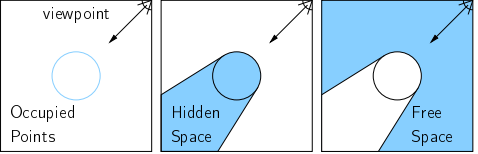
\includegraphics[width=0.9\linewidth]{\FIGDIR/10_Lidar_sets1.PNG} 
    \caption{Space type definitions}
    \label{fig:Spacetypes}
    \end{subfigure}
    \begin{subfigure}{0.5\textwidth}
    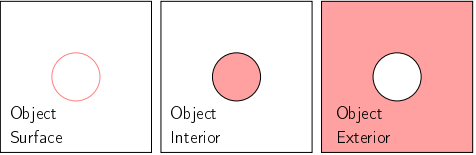
\includegraphics[width=0.9\linewidth]{\FIGDIR/11_Lidar_sets2.PNG}
    \caption{Object properties definitions}
    \label{fig:ObectProperties}
    \end{subfigure}
    \caption{Six spaces of interest \cite{yapo2008probabilistic}}
    \label{fig:Spaces of interests}
 \end{figure}
 
\noindent  Because of real-time obstacle avoidance it is necessary to introduce following terminology:
 \begin{enumerate}
 \item \textit{Occupied points} - points which have been detected by LiDAR (also addressed as visible points).
 \item \textit{Hidden space} - space which is hidden behind occupied points, from viewpoint it is uncertain what is in that space. 
 \item \textit{Free space} - space which is visible from viewpoint and it is not occupied by known objects.
 \item \textit{Object surface} - detected and undetected object surface
 \item \textit{Object interior} - occupied space by object.
 \item \textit{Object exterior} - free space around known objects.
 \end{enumerate}
 Existing method for space segregation \cite{yapo2008probabilistic} can yeld to following definition.
 \begin{definition}[Accessible space]\label{def:accessibleSpace}
    Consider known space $S$ as space explored by sensor (it can have different viewpoint along previous 3D trajectory).
    Intersection between \textit{object exterior} $S_E$ and \textit{free space}$S_F$ gives us \textit{Accessible space}.
    \begin{equation}
        S_A = S_E \cap S_F
    \end{equation}
 \end{definition}
 
 \noindent Accessible space $S_A$ (\ref{def:accessibleSpace}) is our bordering limitation for reachable space of system $R(\tau,t_0,\vec{x_0})$ (def. \ref{def:reachset01}.); 